\chapter{Submodularity, coverage, summarisation}
\label{cap:submodularity}

In this chapter we only provide an overview of what submodularity is, why it is
useful and how it can be applied to summarisation. If you are interested in a
deeper understanding of submodular functions and their many other use-cases,
you can read survey \cite{krause2012submodular} on \emph{submodular function
maximisation}.

\section{Submodular functions}
\label{sec:submod-functions}

In this section we introduce what are submodular functions and why they are
important. We also offer a couple of examples to shed some light on how these
functions behave. Note that we will refer to these examples from some of the
other sections.

\subsection{Definitions}

\begin{definition}[Submodularity]
  \label{def:submodularity}
  A set function \(f : 2^D \to \R\) is submodular iff
  \(\forall S, T \text{ such that } S \subseteq T \subseteq D
    \text{ and } \forall d \in D \setminus T\) we have
  \[f(S \cup {d}) - f(S) \geq f(T \cup {d}) - f(T).\]
\end{definition}
Intuitively this means that a new element's impact can never be higher in the
future than it currently is, an effect also knows as \emph{diminishing returns}.

\begin{definition}[Monotonicity]
  \label{def:monotonicity}
  A set function \(f : 2^D \to \R\) is monotone iff
  \(\forall S, T \text{ such that } S \subseteq T \subseteq D\) we have
  \[f(S) \leq f(T) \text{ and } f(\emptyset) = 0.\]
\end{definition}

From Definition~\ref{def:submodularity} and Definition~\ref{def:monotonicity}
we derive Proposition~\ref{def:mono-submod} \cite{nemhauser1978analysis}.
\begin{proposition}[Monotone submodular]
  \label{def:mono-submod}
  A set function \(f : 2^D \to \R\) is monotone submodular iff
  \(\forall S, T \text{ such that } S \subseteq T \subseteq D
    \text{ and } \forall d \in D\) we have
  \[f(S \cup {d}) - f(S) \geq f(T \cup {d}) - f(T).\]
\end{proposition}
Note that in this case we also allow \(d \in T\).
In Figure~\ref{fig:submodularity} we offer a visual representation of what
submodularity means.

\begin{figure}
  \centering
  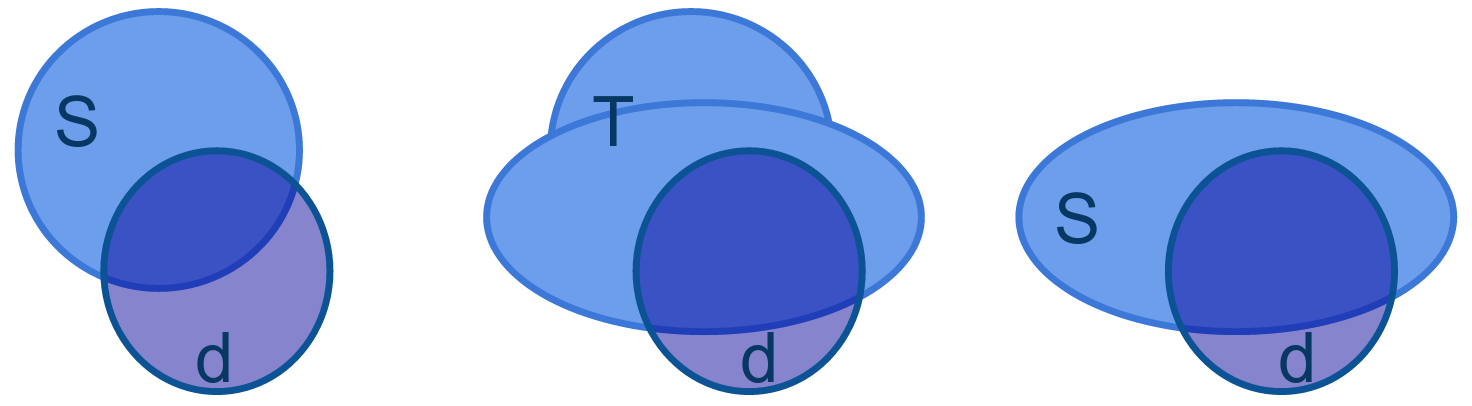
\includegraphics[width=0.9\textwidth,natwidth=1472,natheight=406]{images/submod.png}
  \caption{Visual representation of submodularity. The area contribution of
  \(d\) is larger when added to set \(S\) then when added to the larger set
  \(T\). The right-most image shows the equality case.}
  \label{fig:submodularity}
\end{figure}

\subsection{Examples and properties}

In this subsection we will discuss only monotone submodular functions --
used in the other sections -- and some of the submodular functions'
properties.

Let \(\D\) be a universe, \(A_1, A_2, \ldots, A_n \subseteq \D\) and \(D = {1,
2, \dots, n}\). We can define several functions \(f : 2^D -> \R\) that are
monotone submodular \cite{krause2012submodular}.
\begin{definition}[Set coverage function]
  \label{def:set-coverage}
  \(f(S) := |\bigcup_{i \in S} D_i|\).
\end{definition}
More generally we can extend the above function as follows.
\begin{definition}[Weighted set coverage function]
  \label{def:weighted-coverage}
  Let \(w : \D \to \R_+\) be a non-negative weight function. \\
  Then \(f(S) := w(|\bigcup_{i \in S} D_i|)\).
\end{definition}
This differs from Definition~\ref{def:set-coverage} in that we can sum
non-constant weights that depend on the selected elements.

A very useful property of submodular functions is that the class of submodular
functions is closed under non-negative linear combinations
\cite{krause2012submodular}.

\begin{proposition}[Closedness under non-negative linear combinations]
\label{prop:linear-combinations}
  Let \(g_1, g_2, \ldots, g_n : 2^D \to \R \) be submodular functions and \(\lambda_1, \lambda_2, \ldots, \lambda_n \in \R_+\). \\
  Then
  \[f(S) := \sum_{i=1}^n \lambda_i g_i(S)\]
  is submodular.
\end{proposition}
This property is important because it allows us to easily construct new
submodular function by combining multiple simpler submodular functions.

\section{Submodular function maximisation}
\label{sec:submod-max}

\subsection{Problem statement}

Given a submodular function \(f\) we are interested in maximising its value on
set \(S\) given some constraints on \(S\). A common constraint on \(S\) is the
\emph{cardinality constraint} which limits the size of set \(S\). Formally,
we are interested in computing:
\begin{equation}
  \label{eq:submod-max}
  \max_{S \subseteq D} f(S) \text{ subject to } |S| \leq k, \text{ for some } k
\end{equation}
Most of the time we are actually interested in computing the set \(S\) that
maximises our function \(f\), so Equation~\ref{eq:submod-max} becomes:
\begin{equation}
  \label{eq:submod-argmax}
  \argmax_{S \subseteq D} f(S) \text{ subject to } |S| \leq k, \text{ for some
  } k
\end{equation}

\subsection{Greedy maximisation}
Optimally solving Equations~\ref{eq:submod-max},~\ref{eq:submod-argmax} for
some function \(f\) is \emph{NP-hard} \cite{krause2012submodular}.
\begin{algorithm}
  \caption{Greedy submodular function maximisation}
  \label{alg:greedy-max}
  \begin{algorithmic}
    \STATE \(S \gets \emptyset\)
    \WHILE{\(|S| < k\)}
      \STATE \(d^* \gets \argmax_{d \in D} \left[ f(S \cup {d}) - f(S)
          \right]\)
      \STATE \(S \gets S \cup {d^*}\)
    \ENDWHILE
    \STATE Answer \(S\)
  \end{algorithmic}
\end{algorithm}
Fortunately, we can devise a \emph{greedy algorithm} that is at most \(1 - 1 /
e\) worse than the best solution for maximising a fixed monotone submodular
function \(f\) \cite{nemhauser1978analysis}.
We present the required steps in Algorithm~\ref{alg:greedy-max} and offer a
visual representation in Figure~\ref{fig:sub-max}.
To speed-up the selection process one can use a \emph{max-heap} structure to
keep track of remaining document candidates; this version of the greedy
algorithm is known as \emph{lazy greedy} \cite{minoux1978accelerated}.

\begin{figure}
  \centering
  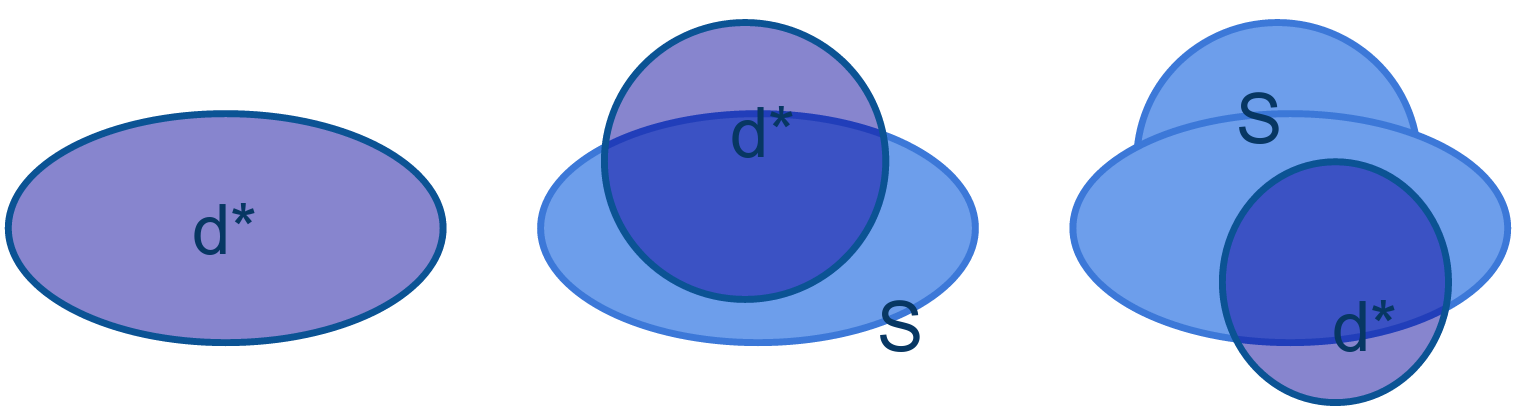
\includegraphics[width=0.9\textwidth,natwidth=1516,natheight=411]{images/sub-max.png}
  \caption{Visual representation of \emph{greedy maximisation}. At each step we
  select the document that adds the highest area contribution.}
  \label{fig:sub-max}
\end{figure}

\subsection{GreeDi protocol}
Given that in this thesis we are interested in applying submodular function
maximisation to a large corpus we need to find a way to transform the
sequential Algorithm~\ref{alg:greedy-max} to run distributively. Fortunately,
there exists a \emph{greedy distributed submodular maximisation} protocol
described in Algorithm~\ref{alg:greedi-dist} that partitions the data into
subsets and then runs Algorithm~\ref{alg:greedy-max} on each individual
partition. This approach has the benefit that it gracefully degrades the
approximation guarantees based on the number of partitions and, more
importantly, for many types of data it offers approximation guarantees close to
the ones offered by the sequential version, also with great experimental
results \cite{mirzasoleiman2013distributed} -- results that are almost identical or very
similar to the sequential algorithm.
\begin{algorithm}
  \caption{Greedy Distributed Submodular Maximisation (GreeDi).
      Adapted from \cite{mirzasoleiman2013distributed} with \(l = k\)}
  \label{alg:greedi-dist}
  \begin{algorithmic}
    \STATE \(D := \)set of all elements
    \STATE \(p := \)number of partitions
    \STATE \(k := \)number of selected elements
  \end{algorithmic}
  \begin{algorithmic}[1]
    \STATE Partition \(D\) into \(p\) sets: \(D_1, D_2, \ldots, D_p\)
    \STATE Run Greedy Algorithm~\ref{alg:greedy-max} on each set \(D_i\) to
        select \(k\) elements in \(T_i\)
    \STATE Merge the answers: \(T = \bigcup_{i=1}^p T_i\)
    \STATE Run Greedy Algorithm~\ref{alg:greedy-max} on T to select the final
        \(k\) elements in \(S\)
    \STATE Answer \(S\)
  \end{algorithmic}
\end{algorithm}

\section{Word coverage}
\label{sec:word-coverage}

One of the basic ways of finding significant multi-document summaries is to
find a good measure for a document's \emph{information coverage}. One such
proposed metric is \emph{word coverage}, a method which argues that covering
words is a good indication of covering information. This method has been used
before in document summarisation and it extends naturally to multi-document
summarisation \cite{sipos2012temporal}.

\subsection{Definition}

Sipos et al \cite{sipos2012temporal} propose a way to adapt a known submodular
function to use word coverage as a information measure. We define this function
in Definition~\ref{def:word-coverage}.
\begin{definition}[Word coverage]
  \label{def:word-coverage}
  Let:
  \begin{align*}
    &D \text{ be a set of documents, } \\
    &W \text{ be a set of all words from all documents in \(D\).}
  \end{align*}
  Then we define:
  \begin{align*}
    &f : 2^D \to \R_+ \\
    &f(S) := \sum_{w \in W} \theta(w) \max_{d \in S} \phi(d, w)
    \,(\forall S \subseteq D)
  \end{align*}
  where:
  \begin{align*}
    &\theta : W \to \R_+ \text{ represents the importance of word \(w\),} \\
    &\phi : D \times W \to \R_+
    \begin{aligned}[t]
      &\text{represents the coverage of word \(w\) in document \(d\)} \\
      &\text{and it is usually chosen to be tf-idf\((d, w)\).}
    \end{aligned}
  \end{align*}
\end{definition}
Remember that we described term-frequency--inverted-document-frequency (tf-idf)
in Section~\vref{sec:tf-idf}. In Figure~\ref{fig:max-phi} we visually explain
the behaviour of taking the maximum of \(\phi(d, w)\) over the selected
documents.

\begin{figure}
  \centering
  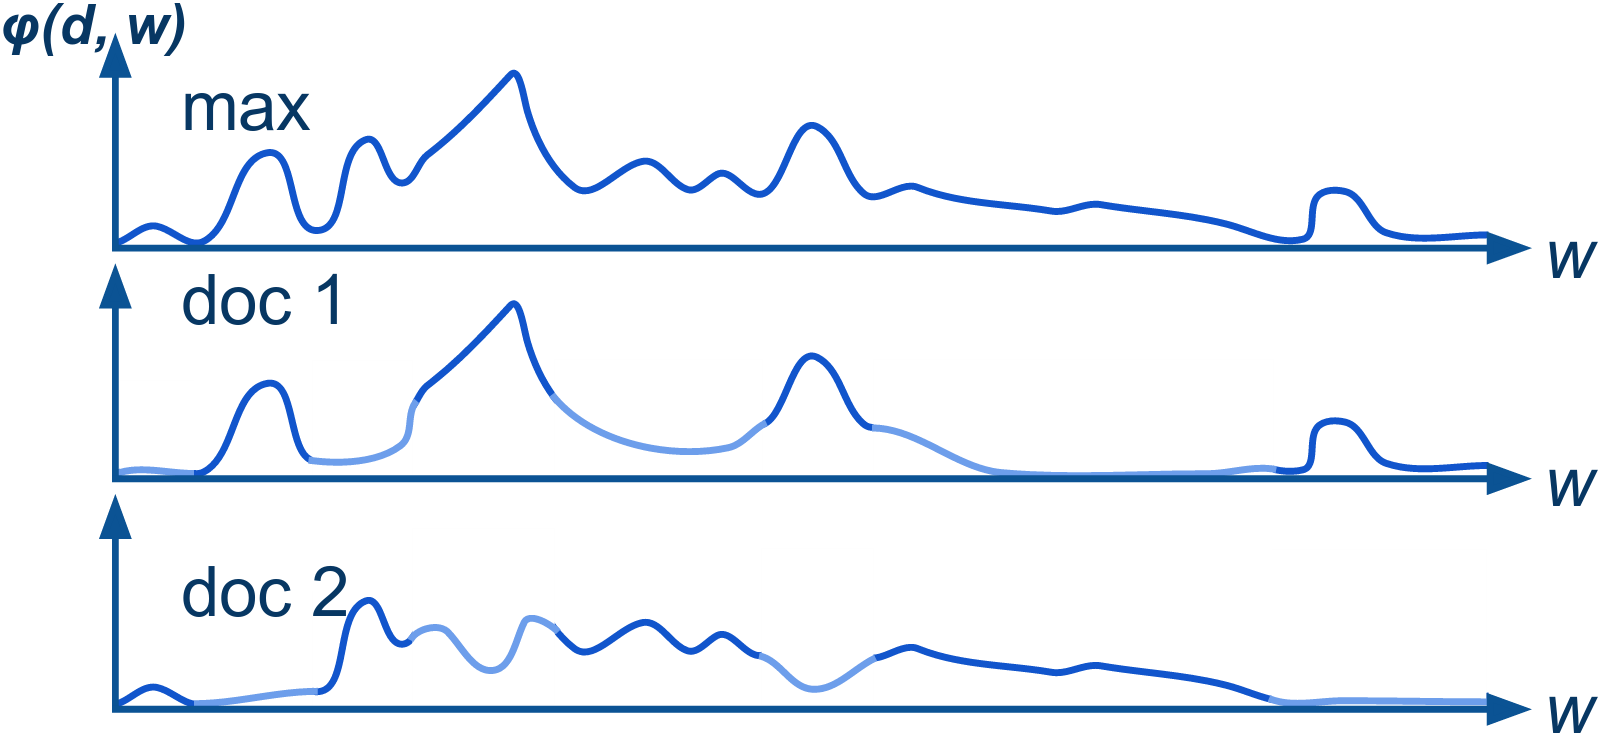
\includegraphics[width=0.9\textwidth,natwidth=1601,natheight=738]{images/max-phi.png}
  \caption{Visual representation of \(\max_{d \in S} \phi(d, w)\). The \(X\)
  axis represents the words and the \(Y\) axis represents the value of \(\phi\)
  for a given document and word. Given two documents, the result of taking for
    each word the maximum value of the two is shown in the \emph{max} plot.}
  \label{fig:max-phi}
\end{figure}

\begin{proposition}
  \label{prop:word-coverage}
  Function \(f\) from Definition~\ref{def:word-coverage} is monotone submodular.
  \begin{proof}
    It is easily proven because taking the maximum of a function over all
    selected documents is monotone submodular. Then we just do a weighted sum
    of submodular functions which is again submodular according to
    Proposition~\ref{prop:linear-combinations}.
  \end{proof}
\end{proposition}

\subsection{Rationale}

The word coverage function defined in Definition~\vref{def:word-coverage}
promotes word diversity while trying to minimize eccentricity. Intuitively,
maximising \(\phi(d, w\), seen as tf-idf, prefers selecting documents that have
a lot of words rarer in the other documents. This promotes diversity, but also
increases the eccentricity of the selected documents. To dampen the
eccentricity of picked documents we introduce \(\theta(w)\) so that we include
the importance of the word in the selection process. This will counterbalance
the eccentricity of words by preferring more common significant
words\footnote{Not to be confused with stop words.}.

\section{Document influence}
\label{sec:doc-influence}

While word coverage captures information well enough, it does not explain how
documents influenced each other nor how the corpus evolved over time. By
capturing document influence in the submodular function, one can use this new
measure to select the most important documents.

\subsection{Definition}

Sipos et al \cite{sipos2012temporal} propose combining two complementary
notions in a single submodular function that takes into account document
influence when scoring an article. We define this function in
Definition~\ref{def:doc-influence}.

Let:
\begin{align*}
  &D \text{ be a set of documents,} \\
  &W \text{ be a set of all words from all documents in \(D\),} \\
  &Y \text{ be a set of all publishing dates of the documents in \(D\),} \\
  &t(d) \text{ be a function that gives the publishing date of document \(d \in
  D\).}
\end{align*}

\begin{definition}[Document influence]
  \label{def:doc-influence}
  We define:
  \begin{align*}
    &f : 2^D \to \R_+ \\
    &f(S) := \sum_{w \in W} \sum_{y \in Y} \theta(w, y)
    \max_{d \in \{d' \in S | t(d') < y\}} \nu(d, w) \,(\forall S \subseteq D)
  \end{align*}
  where:
  \begin{align*}
    &\theta : W \times Y \to \R_+
    \begin{aligned}[t]
      &\text{represents the importance of word \(w\) in year \(y\)} \\
      &\text{and it used to measure the \emph{spread} of the word,}
    \end{aligned} \\
    &\phi : D \times W \to \R_+ \text{ represents the \emph{novelty} of word
    \(w\) in document \(d\).}
  \end{align*}
\end{definition}

The same authors \cite{sipos2012temporal} also define \emph{word spread} and
\emph{document novelty} that are used above in
Definition~\ref{def:doc-influence}.
Let:
\begin{align*}
  &\phi : D \times W \to \R_+
  \begin{aligned}[t]
    &\text{be the coverage of word \(w\) in document \(d\),} \\
    &\text{usually chosen to be tf-idf\((d, w)\).}
  \end{aligned}
\end{align*}

\begin{definition}[Word spread]
  \label{def:word-spread}
  We define:
  \begin{align*}
    &\theta : W \times Y \to \R_+
    &\theta(w, y) = \sum_{d \in \{d' \in D | t(d) = y\}} \phi(d, w)
  \end{align*}
\end{definition}

\begin{definition}[Document novelty]
  \label{def:doc-novelty}
  We define:
  \begin{align*}
    &\nu : D \times W \to \R_+ \\
    &\nu(d, w) = \max \left\{ 0, \min_{d' \in \mathcal{N}(d)}
      \left\{ \phi(d, w) - \phi(d', w) \right\} \right\}
  \end{align*}
  where:
  \begin{align*}
    &\mathcal{N}(d)
    \begin{aligned}[t]
      &\text{is a set representing the k-nearest neighbours of
    document \(d\)} \\
      &\text{from the given corpus \(D\).}
    \end{aligned}
  \end{align*}
\end{definition}

\begin{proposition}
  Function \(f\) from Definition~\ref{def:doc-influence} is monotone submodular.
  \begin{proof}
    Similar to Proposition~\ref{prop:word-coverage} \cite{sipos2012temporal}.
  \end{proof}
\end{proposition}
\subsection{Rationale}

In order to measure \emph{document influence} we have to find suitable metrics
that achieve this exact task. Sipos et al \cite{sipos2012temporal} propose two
metrics:
\begin{itemize}
  \item word spread
  \item document novelty
\end{itemize}
that together achieve our purpose of measuring influence and as such find the
most important, valuable documents.
In Figure~\ref{fig:submodularity} we offer a visual representation of
\emph{document influence} function.

\begin{figure}
  \centering
  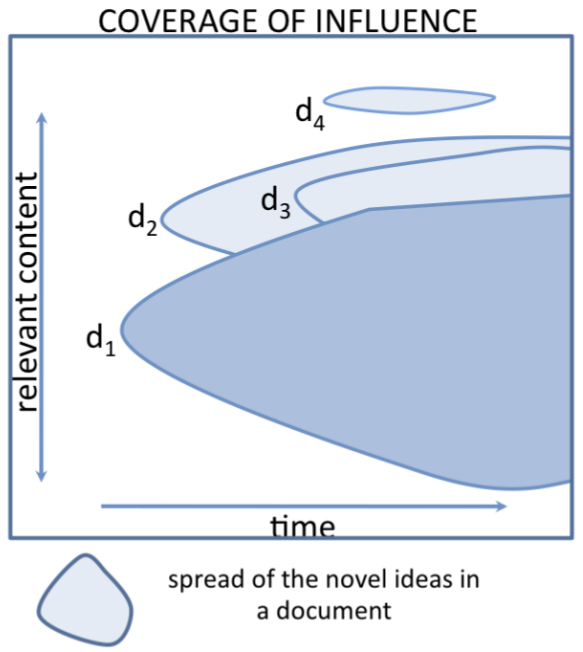
\includegraphics[width=0.5\textwidth,natwidth=583,natheight=652]{images/doc-infl.png}
  \caption{Visual representation of \emph{document influence} submodular
  function. Image source: \cite{sipos2012temporal}}
  \label{fig:doc-infl}
\end{figure}

\subsubsection{Word spread}

The idea of \emph{word spread} stems from viewing words not just as static
concepts, but as ideas that evolve over time.
To be able to do this one has to extend the concept of \emph{word importance}
introduced in Definition~\vref{def:word-coverage} to depend not only the word
itself, but also on the year that word is to be considered.
This is a valuable insight because as humans when we talk about a field -- for
example, neural networks -- we would value that term differently depending on
the year we are in. If we were in 1980, it would be an exciting new idea that
will manage to solve all the difficult \acl{AI} problems, if we were in the
1990s, it would have been an idea that cannot solve any of the harder problems,
while today we view the neural networks field very promising again.
In a nutshell \emph{word spread} aims to capture what are the important
concepts on each particular date. It is important to note that this date is
open to different granularities: which can be anything from hour granularity
(or smaller) up to year granularity (or larger).

\subsubsection{Document novelty}

While the formal definition of \emph{document novelty} might look a little more
complicated, the intuition behind it is really simple: we want to minimize
counting the same concepts -- mentioned in multiple documents -- multiple
times.
For example, when considering published papers, if we already selected \(3\)
very good documents, we want to lower the \emph{novelty score} of a survey
paper that discusses the same \(3\) papers.
This is true for \emph{Wikipedia} as well, where one can find (human-written)
general articles that offer an overview of a broad topic and where each section
links to another page that only discusses that particular sub-topic.

